% Reconstructed from the submitted PDF (IEEEtran conference format).
% Clean manuscript: revision wrappers retain their content without color markup.
% Text that the revision replaced is not kept; the sentence it replaces is named in a "% REPLACES:" comment.
\documentclass[conference]{IEEEtran}
\usepackage{amsmath,amssymb}
\usepackage{graphicx}
\usepackage{xcolor}
\usepackage{booktabs}
\usepackage{array}
\usepackage{url}
\usepackage[T1]{fontenc}
\usepackage{listings}
\usepackage{cite}

\newcommand{\new}[1]{{#1}}
\newenvironment{newtext}{\begingroup}{\endgroup}
\newcommand{\llvmmca}{\texttt{llvm-mca}}
\newcommand{\Rsq}{R^{2}}
\newcommand{\rd}[1]{{#1}}
\newenvironment{rdblock}{\begingroup}{\endgroup}
% Final original2000 test metrics, all three seeds (42,43,44).
% Updated 2026-11-10 from completed training results; full-test values are reported separately.
\newcommand{\CBIPCR}{0.860}
\newcommand{\CBIPCRCell}{.8597\,\pm\,.0052}
\newcommand{\CBIPCMAE}{0.195}
\newcommand{\CBIPCMAECell}{.195\,\pm\,.005}
\newcommand{\CBIPCRawR}{0.870}
\newcommand{\CBIPCRawRCell}{.8695\,\pm\,.0051}
\newcommand{\CBJointR}{0.876}
\newcommand{\CBJointRCell}{.8759\,\pm\,.0069}
\newcommand{\CBJointMAE}{0.188}
\newcommand{\CBJointMAECell}{.188\,\pm\,.004}
\newcommand{\CBJointRawR}{0.887}
\newcommand{\CBJointRawRCell}{.8874\,\pm\,.0070}
\newcommand{\UXIPCR}{0.890}
\newcommand{\UXIPCRCell}{.8898\,\pm\,.0044}
\newcommand{\UXIPCMAE}{0.177}
\newcommand{\UXIPCMAECell}{.177\,\pm\,.003}
\newcommand{\UXIPCRawR}{0.896}
\newcommand{\UXIPCRawRCell}{.8958\,\pm\,.0043}
\newcommand{\UXJointR}{0.891}
\newcommand{\UXJointRCell}{.8912\,\pm\,.0021}
\newcommand{\UXJointMAE}{0.180}
\newcommand{\UXJointMAECell}{.180\,\pm\,.002}
\newcommand{\UXJointRawR}{0.895}
\newcommand{\UXJointRawRCell}{.8947\,\pm\,.0022}


\begin{document}

\title{Source-Level Static Performance Estimation\\through Assembly-Supervised Learning}
\author{\IEEEauthorblockN{Lirong Yi}
\IEEEauthorblockA{Chalmers University of Technology\\Gothenburg, Sweden}}
\maketitle

\begin{abstract}
Estimating performance characteristics directly from source code can provide execution-related information early in software development. We present an assembly-supervised framework that predicts static instructions per cycle (IPC) from C functions. Source--assembly alignment supplies implementation information during training, while IPC regression organizes the source representation around labels generated by \llvmmca{} under a Skylake scheduling model. An instruction-aware (IA) tokenizer preserves whole opcodes and abstract operand classes within a compact assembly sequence. Prediction requires only the source encoder and a linear readout. On a fixed 2,000-function sample, a 7.52M-parameter compact encoder improves $\Rsq$ from 0.607 with IPC-only supervision to 0.752 with joint training. IA improves on BPE assembly encoding, which reaches 0.734. Evaluation on all 17,301 test functions extends the supervision benefit to CodeBERT and UniXcoder, with gains retained on 12,600 functions after filtering near-duplicates of training inputs. Every matched seed improves in $\Rsq$ for all three encoders on both expanded evaluation sets. Mixed-view training also supports prediction when declarations needed for compilation are missing, reaching $\Rsq=0.660$ on 1,136 declaration-stripped functions. Only 2.8\% of these inputs pass compilation checks. These results establish paired assembly as useful training information for source-level static performance estimation across compact and pretrained representations.
\end{abstract}

\begin{IEEEkeywords}
static performance prediction, instructions per cycle, source code representation, assembly supervision, contrastive learning
\end{IEEEkeywords}

\section{Introduction}
Estimating performance characteristics directly from source code can provide execution-related information early in software development. Developers inspect functions, compare implementations, and explore repositories at the source level. Associating these functions with execution-related estimates adds a numerical perspective to those activities and helps direct further analysis. Early prediction has been explored for worst-case execution time~\cite{bonenfant2017wcet}, functional-test execution time~\cite{samoaa2022tep}, and LLVM-based timing analysis~\cite{xu2025preti}.

\begin{newtext}
Source-level analysis applies when a function is inspected separately from its surrounding declarations. A retrieved function or isolated excerpt may omit type definitions, macros, and forward declarations needed for compilation. Analysis of partial programs has a long history~\cite{dagenais2008partial}, and code snippets taken from Q\&A sites are often not compilable~\cite{terragni2016csnippex}. Missing declarations can prevent compilation, leaving a compile-then-analyze pipeline without the assembly required by its analyzer. A source-level predictor can still produce an estimate directly from the available code, drawing on implementation information acquired during training. We study this setting through a predictor of static instructions per cycle (IPC), with labels supplied by \llvmmca{} under a fixed Skylake scheduling model.
\end{newtext}

The challenge is to connect the information expressed in source code with the behavior of its compiled implementation. Source exposes variables, expressions, and control structures; assembly exposes instructions and operands that use processor execution resources. A scalar IPC label identifies the numerical target, while the paired assembly reveals a structured implementation associated with that label. Their combination gives the source encoder both a target and an additional view from which to learn it.

\begin{newtext}
The framework combines source--assembly contrastive alignment with source-side IPC regression. We study a compact Transformer trained from scratch and extensions to pretrained source encoders. An instruction-aware (IA) tokenizer represents assembly through whole opcodes and abstract operand classes, allowing more instructions to fit within the sequence budget. After training, a Ridge readout predicts IPC from frozen source embeddings. The assembly branch supplies training information; the prediction path retains the source encoder and a linear readout.

Controlled comparisons on 2,000 test functions show that the compact joint model reaches $\Rsq=0.752$, compared with 0.607 for IPC-only supervision and 0.488 for alignment alone. IA improves on BPE assembly encoding (0.734), while source-count gradient boosting reaches 0.585 with all training labels. We apply the same alignment principle to CodeBERT and UniXcoder under a shared 9,762-update budget.

On the full 17,301-function test partition, joint supervision improves every matched seed for all three source encoders. These gains persist after filtering near-duplicates of training functions, leaving 12,600 test inputs. This connects the compact-model ablations to a broader result: compiled implementations supply useful training information for both task-trained and pretrained source representations. The compact instantiation also provides a lightweight prediction path, with its encoder and readout taking 1.79\,ms per pretokenized query on an A100.

We then extend the framework to functions that cannot be compiled in isolation because declaration context is missing. Mixing complete and declaration-stripped inputs during training yields $\Rsq=0.660$ on 1,136 declaration-stripped test functions while retaining 0.739 across all 2,000 complete test inputs. Only 2.8\% of the stripped functions pass compilation checks, yet the model produces predictions directly from their source. The source interface therefore makes static IPC estimates available when compilation cannot supply assembly to the analyzer.

The paper makes three contributions:
\begin{itemize}
\item An assembly-supervised framework for source-level static IPC prediction. Joint implementation alignment and numerical supervision strengthen source representations across compact and pretrained encoders.
\item An instruction-aware assembly encoding that increases sequence coverage and improves the performance signal learned by the source encoder.
\item An evaluation of supervision and assembly encoding across compact and pretrained source encoders, including full-partition prediction, training-overlap filtering, inference cost, and prediction with missing declaration context.
\end{itemize}
\end{newtext}

\begin{table*}[t]
\caption{Positioning of related approaches by prediction input and objective.}
\label{tab:related}
\centering\small
\begin{tabular}{p{5.2cm}p{5.2cm}p{6.2cm}}
\toprule
Research line / examples & Prediction or downstream input & Prediction target / learning objective\\
\midrule
Early WCET~\cite{bonenfant2017wcet}, TEP-GNN~\cite{samoaa2022tep} & Source features / code structure & Worst-case execution time; functional-test execution time\\
GFTrans~\cite{li2026gftrans} & Source-derived flow paths and code features & Runtime-category prediction\\
DeepTune~\cite{cummins2017deeptune} & Source tokens & Heterogeneous device mapping and thread coarsening\\
PrETi~\cite{xu2025preti} & LLVM simulation features & Early execution-time prediction\\
Ithemal~\cite{mendis2019ithemal}, GRANITE~\cite{sykora2022granite} & Basic-block assembly & Learned basic-block throughput prediction\\
uiCA~\cite{abel2022uica}, Facile~\cite{abel2023facile}, OSACA~\cite{laukemann2019osaca} & Assembly blocks or kernels & Analytical throughput modeling; critical-path analysis\\
BHive~\cite{chen2019bhive}, DiffTune~\cite{renda2020difftune} & Basic-block assembly with measured throughput & Hardware-measured throughput benchmark; learning \llvmmca{} parameters\\
IR2Vec~\cite{ir2vec2020}, ProGraML~\cite{cummins2021programl}, PERFOGRAPH~\cite{tehranijamsaz2023perfograph}, MIREncoder~\cite{dutta2024mirencoder} & LLVM IR representations & Program representation learning for analysis and optimization\\
PerfVec~\cite{li2024perfvec}, Concorde~\cite{nasr2025concorde} & Execution-derived representations & Program / architecture representation learning; CPU performance modeling\\
ContraBin~\cite{zhang2022pre}, CLAP~\cite{wang2024clap} & Binary / assembly embeddings & Cross-modal representation learning for binary analysis\\
LLM Compiler~\cite{cummins2024llmcompiler} & LLVM IR and assembly & Pretrained language models for compiler tasks\\
PPA~\cite{dagenais2008partial}, CSnippex~\cite{terragni2016csnippex} & Incomplete programs / code snippets & Static analysis and compilable-code synthesis for partial code\\
\textbf{This study} & \textbf{Source code at inference} & \textbf{Static IPC prediction; assembly-supervised source representation learning}\\
\bottomrule
\end{tabular}
\end{table*}

\section{Background and Related Work}
\subsection{Source-Level Performance Prediction}
Bonenfant et al.~\cite{bonenfant2017wcet} investigated machine learning for early worst-case execution time prediction from C source, motivated by development stages where executable-level timing information is difficult to obtain. TEP-GNN~\cite{samoaa2022tep} uses flow-augmented abstract syntax trees and graph neural networks to predict functional-test execution times in Java projects. More recently, GFTrans~\cite{li2026gftrans} combines source-derived control- and data-flow paths with explicit code features to classify C functions into four runtime categories. Our framework targets continuous static IPC prediction and uses compiled assembly as additional supervision for the source representation.

PrETi~\cite{xu2025preti} predicts execution time using features extracted through LLVM-based execution-flow, cache, and branch simulation, together with historical timing data. Our framework uses compilation and \llvmmca{} during corpus construction, then transfers information from that analysis into a source encoder. Its static IPC target captures the instruction-stream behavior represented by the recorded processor configuration. 

B\"ock et al.~\cite{bock2023domain} evaluated source-based performance comparison across programming tasks and an industrial game-development domain, highlighting the importance of task and domain. We study whether paired assembly can strengthen that connection for a source-level static IPC predictor.

\subsection{Instruction-Level Performance Models}
Static instruction-stream models connect machine instructions to processor behavior. \llvmmca{}~\cite{llvm_mca} uses LLVM scheduling information to estimate execution and resource behavior. OSACA analyzes assembly kernels, including critical paths and loop-carried dependencies~\cite{laukemann2019osaca}. uiCA models basic-block throughput on recent Intel microarchitectures~\cite{abel2022uica}, while Facile decomposes throughput prediction into analytical bottleneck models~\cite{abel2023facile}. BHive~\cite{chen2019bhive} supplies hardware-measured basic-block throughput for validating such models, including \llvmmca{}, and DiffTune~\cite{renda2020difftune} learns \llvmmca{} parameters from hardware measurements.

Learned models capture this relationship from instruction-level training data. Ithemal~\cite{mendis2019ithemal} learns basic-block throughput from assembly using a recurrent model. GRANITE~\cite{sykora2022granite} represents basic blocks as graphs with structural and data dependencies and uses a graph neural network for throughput prediction. Concorde~\cite{nasr2025concorde} combines analytical performance distributions with learned models for CPU performance prediction and architectural sensitivity analysis.

\subsection{Performance-Oriented Representations}
DeepTune~\cite{cummins2017deeptune} learns optimization heuristics from raw code for heterogeneous device mapping and GPU thread coarsening. IR2Vec~\cite{ir2vec2020} constructs embeddings from LLVM intermediate representations, while PERFOGRAPH~\cite{tehranijamsaz2023perfograph} enriches IR graphs with numerical information and aggregate data structure representations for performance optimization and program analysis. ProGraML~\cite{cummins2021programl} represents programs as graphs over LLVM IR and evaluates them on data-flow analysis and compiler optimization tasks.

MIREncoder~\cite{dutta2024mirencoder} combines IR-token and graph representations through multimodal pretraining, including IR--graph matching. Its reusable embeddings support several performance optimization tasks, including device mapping, thread coarsening, and loop vectorization. Our framework brings a related implementation-informed learning strategy to a source-input numerical predictor, using paired assembly and IPC labels to shape the source encoder.

PerfVec~\cite{li2024perfvec} learns program and microarchitecture representations for performance modeling, deriving program representations from instruction execution traces. We train source embeddings with paired assembly and a static numerical label, then evaluate their target information through a common Ridge readout.

\subsection{Cross-Modal Code Learning}
Asm2Vec~\cite{ding2019asm2vec} learns lexical and function-level assembly representations for binary clone search. PalmTree~\cite{palmtree2021} learns instruction embeddings through assembly-oriented pretraining objectives, and Nova~\cite{jiang2025nova} combines hierarchical attention and contrastive objectives for assembly generation and understanding. LLM Compiler~\cite{cummins2024llmcompiler} pretrains language models on LLVM IR and assembly for compiler tasks. Our IA tokenizer exposes whole opcodes and operand categories to the assembly encoder.

Cross-modal supervision links low-level code to other views of a program. ContraBin~\cite{zhang2022pre} trains binary representations against anchored source and comment encoders. CLAP~\cite{wang2024clap} aligns assembly with natural-language semantic explanations to learn transferable binary representations. Our framework directs the information toward the source branch: alignment with compiled implementations enriches a trainable source encoder, and IPC regression shapes its representation for numerical performance prediction. Using an additional view during training also relates to learning using privileged information~\cite{vapnik2015privileged}, where richer training information supports a decision rule operating on the primary input.

CodeBERT~\cite{feng2020codebert} and UniXcoder~\cite{unixcoder2022} provide general pretrained code encoders that can be adapted to IPC using source-only regression. Our experiments compare IPC-only adaptation with assembly-supervised adaptation of both pretrained encoders, alongside a compact encoder trained from scratch on the task corpus. Table~\ref{tab:related} summarizes how these research lines differ in their prediction inputs and objectives.


\section{Method}
\subsection{Overview}
Each training example is a triplet $(S_i,A_i,y_i)$ containing a C function, its compiled x86-64 assembly, and a static IPC label generated by \llvmmca{}. For a compilation and processor-analysis configuration $c$, we learn a source predictor of $y_c(S)$. IPC is the analyzed instruction count divided by the simulated cycle count, characterizing instruction execution under the selected processor scheduling model and analysis region.

Figure~\ref{fig:framework} illustrates the paired data with a maximum function, its compiled instructions, and its recorded static IPC of 2.96. The source and assembly encoders map their inputs into a shared 128-dimensional space. Contrastive learning associates each source function with its compiled instruction stream, and a linear IPC head encourages the source embedding to retain the numerical performance signal. After training, the frozen source encoder supplies embeddings to a separately fitted Ridge readout.

\begin{figure*}[t]
\centering
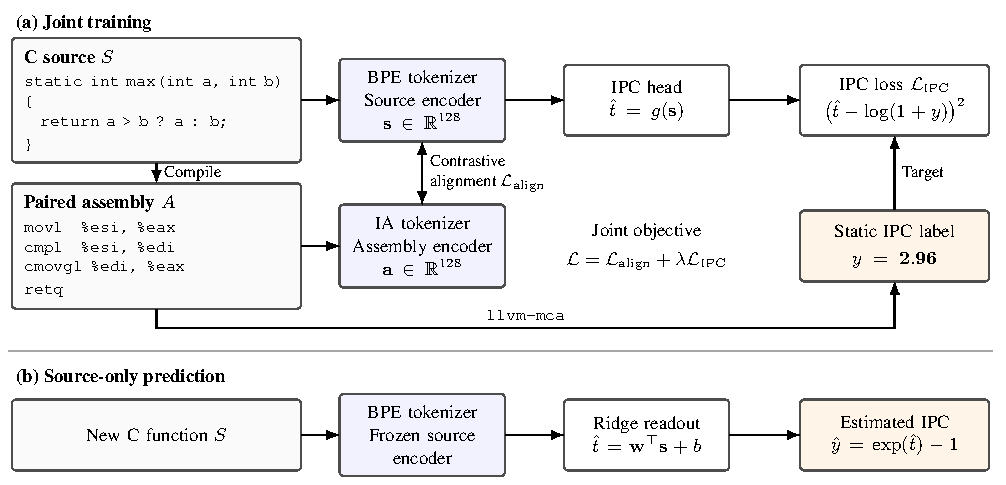
\includegraphics[width=0.92\textwidth]{figures/framework.pdf}
\caption{Assembly-supervised source-level IPC estimation. (a) A training-corpus example links a C maximum function to its four compiled instructions and recorded static IPC label, $y=2.96$. Source--assembly alignment and IPC regression jointly train the source representation. (b) A new function is encoded from source and mapped to an IPC estimate through the frozen encoder and Ridge readout. Source boilerplate, declaration attributes, and assembly directives are omitted from the example.}
\label{fig:framework}
\end{figure*}

\subsection{Instruction-Aware Tokenization}
IA represents assembly as a sequence of opcode and operand-category tokens. Each instruction begins with a whole-opcode token. Register operands become typed classes, including general-purpose widths and SIMD classes; numeric immediates and memory displacements receive abstract markers. The encoder thus sees recurring patterns shared by instructions that differ in concrete register allocation or numeric values.

For example, \texttt{addq \%rax, \%rbx} becomes the token sequence \texttt{[ADDQ] [GPR64] [GPR64]}. The instruction \texttt{movq 8(\%rax), \%rbx} yields \texttt{[MOVQ] [MEM] [GPR64] [GPR64]}. Normalization preserves operand order. The tokenizer ignores assembler directives, standalone labels, and inline comments, and uses an unknown token for unrecognized opcodes. The resulting vocabulary contains 254 entries, including special tokens.

Whole-opcode tokens and abstract operands expose recurring instruction patterns while preserving register-width and vector-class distinctions. This representation covers longer instruction streams within the shared 512-token budget, supplying alignment with more of each paired implementation.

\subsection{Encoders}
The compact instantiation uses a 16,384-entry BPE source vocabulary. Both modalities have a maximum sequence length of 512, including boundary tokens, and longer inputs are truncated. Each compact encoder consists of token embeddings and learned positional embeddings followed by four pre-LayerNorm Transformer layers, with hidden dimension 256, four attention heads, feed-forward dimension 1,024, and dropout 0.1. Masked mean pooling excludes padding positions; a final LayerNorm and bias-free linear projection produce the 128-dimensional embedding.

Writing the source and assembly embeddings as $\mathbf{s}_i=f_S(S_i)$ and $\mathbf{a}_i=f_A(A_i)$, the source branch contains 7,517,696 parameters. The joint IA training model, including the linear IPC head, contains approximately 10.91M parameters. Source-only prediction retains the source branch and a linear readout.

\subsection{Joint Training}
For a batch of $B$ pairs, cosine similarity defines the cross-modal scores
\begin{equation}
q_{ij}=\frac{\langle \bar{\mathbf{s}}_i,\bar{\mathbf{a}}_j\rangle}{\tau},\qquad \bar{\mathbf{s}}_i=\mathbf{s}_i/\lVert\mathbf{s}_i\rVert_2,
\end{equation}
with analogous normalization for assembly and temperature $\tau=0.05$. The positive match for source $i$ is assembly $i$; other batch entries provide negatives. We minimize the mean of source-to-assembly and assembly-to-source cross-entropies, using uniform label smoothing of 0.05. This symmetric contrastive objective follows the paired-instance learning principle of InfoNCE~\cite{oord2018representation}.

A linear head $g$ predicts the transformed target $t_i=\log(1+y_i)$ from $\mathbf{s}_i$. The complete objective is
\begin{equation}
\mathcal{L}=\mathcal{L}_{\mathrm{align}}+\lambda\frac{1}{B}\sum_{i=1}^{B}\bigl(g(\mathbf{s}_i)-t_i\bigr)^2 .
\label{eq:joint}
\end{equation}
The paired-instance objective asks the source representation to distinguish its compiled implementation from other implementations in the batch, providing supervision even when functions have similar IPC labels. Regression directs the representation toward distinctions relevant to the numerical target. The supervision ablation removes one term at a time to assess their combined benefit.

We calibrate the regression weight using training-label variance,
\begin{equation}
\lambda=\beta\,\frac{\operatorname{Var}(y)}{\operatorname{Var}(\log(1+y))}.
\end{equation}
This expresses candidate regression weights on a comparable target-variance scale when selecting between raw and transformed labels. Validation selection yields $\beta=0.6$ with the transformed target, corresponding to $\lambda=5.9905$. IA and BPE use the same selected target and weight in the final comparison.

\subsection{Source-Level Prediction}
The final readout maps frozen source embeddings to transformed IPC. Given a fixed set $\mathcal{P}$ of labeled training examples, Ridge fits
\begin{equation}
\min_{\mathbf{w},b}\sum_{i\in\mathcal{P}}(\mathbf{w}^{\top}\mathbf{s}_i+b-t_i)^2+\alpha\lVert\mathbf{w}\rVert_2^2,
\end{equation}
with $\alpha=1$ and an unpenalized intercept. No embedding standardization is applied. The output in IPC units is $\hat{y}=\exp(\mathbf{w}^{\top}\mathbf{s}+b)-1$.

The regression head shapes the representation during joint training; the separately fitted Ridge readout turns that representation into the final predictor. Using the same readout across encoders also makes their performance information directly comparable. 

\begin{newtext}
\subsection{Mixed-View Training}
\label{sec:aug}
We construct a declaration-stripped input by retaining the function definition from the \texttt{\_\_attribute\_\_((used))} marker and removing its preceding context. The marker occurs in 1,136 of the 2,000 test functions. During joint training, each source is replaced by its declaration-stripped input with probability $p=0.5$ when one exists. Functions without the marker remain unchanged. Assembly partners, IPC labels, architecture, optimizer, and update schedule retain the original configuration. This setting relates to partial-program analysis~\cite{dagenais2008partial} and compilable-snippet synthesis~\cite{terragni2016csnippex}, which recover missing context before analysis; our predictor instead estimates the target directly from the incomplete source.

We call the resulting model the \emph{mixed-view model}; the original joint model uses complete inputs throughout training. Both predict the label of the original compiled implementation, so declaration-stripped inputs test prediction under controlled context removal. The primary Ridge readout uses complete inputs of the same 5,000 training functions; a secondary readout adds their declaration-stripped inputs as extra observations.
\end{newtext}

\section{Experimental Setup}
\subsection{Data}
The corpus consists of AnghaBench-derived C functions~\cite{da2021anghabench}, compiled into x86-64 assembly using an LLVM pipeline and paired with \llvmmca{} IPC labels. The original partitions contain 309,913 training functions, 17,150 validation functions, and 17,301 test functions. We retain these partitions and use the same record identities across all model comparisons.
\begin{newtext}
Re-running \llvmmca{} 18.1.8 with \texttt{-mcpu=skylake} and 100 iterations reproduced the recorded IPC labels to their stored precision on 2,346 functions with self-contained assembly from the full 17,301-function test partition. All labels refer to this fixed analysis configuration.
\end{newtext}

For encoder evaluation, a fixed sample of 5,000 training functions supplies the Ridge fitting set. Validation uses the first 2,000 records in the original validation partition. Controlled ablations, feature references, and declaration-removal experiments use the first 2,000 test records; expanded evaluation uses the full 17,301-function partition. These samples are fixed before the final model comparisons. Model initialization and training order vary across seeds, while the readout fitting set and evaluation functions remain unchanged. 

\subsection{Training}
The compact encoders train from scratch for 9,762 parameter updates with batch size 256, including 256 paired examples in each contrastive loss. Optimization uses AdamW, learning rate $10^{-3}$, weight decay 0.01, and gradient clipping at 0.5. The schedule has 200 warmup steps followed by cosine decay on a 10,000-step horizon, with a minimum multiplier of 0.1. The compact models use bfloat16 training on NVIDIA A100-SXM4-40GB GPUs. All encoder comparisons use 9,762 updates with effective batch size 256, corresponding to approximately 8.06 passes over the training set. Pretrained-model experiments use NVIDIA GH200 GPUs with PyTorch 2.9.1. 

We select the IPC target and regression weight using validation probe $\Rsq$. Raw and log-transformed targets are evaluated with base weights 0.05, 0.15, 0.3, and 0.6 for each assembly representation. Candidates receive 2,000 updates; the two highest-validation candidates per representation continue to the full budget before final selection. The selected configuration is fixed for seeds 42, 43, and 44 and for the supervision ablations.

\subsection{Baselines and Ablations}
\textbf{Pretrained source encoders.} CodeBERT~\cite{feng2020codebert} and UniXcoder~\cite{unixcoder2022} are adapted under two conditions: IPC-only regression and joint assembly alignment with IPC regression. Each uses its native tokenizer, a maximum input length of 512, masked mean pooling over the complete 768-dimensional representation, and a linear IPC head. UniXcoder uses the encoder-only sequence format. Both conditions update the entire source encoder and head. The source encoders contain 124,055,040 and 125,339,136 parameters, respectively.

The joint condition adds the same IA assembly encoder used by the compact model and a bias-free source projection from 768 to 128 dimensions. The projection supplies the alignment embedding, while the IPC head operates on the full 768-dimensional source representation. Its objective is $\mathcal{L}_{\mathrm{MSE}}+\gamma\mathcal{L}_{\mathrm{align}}$, with the same temperature, label smoothing, and 256 paired examples as the compact joint model. The source architecture and IPC head remain identical between conditions. At prediction time, the assembly encoder and alignment projection are discarded; the common Ridge readout uses frozen 768-dimensional source embeddings.

Both pretrained conditions use bfloat16, 9,762 updates, effective batch size 256, and the compact model's AdamW decay, clipping, and step-based schedule. Microbatches contain 16 functions. A two-pass gradient cache preserves the full-batch objective by replaying encoder forward passes with identical dropout randomness.

Selection uses validation probe $\Rsq$ at seed 42. For each encoder, learning rates $10^{-5}$, $2\times10^{-5}$, and $5\times10^{-5}$ receive 2,000 IPC-only updates. The two leading candidates continue from their checkpoints to 9,762 updates. Both encoders select $5\times10^{-5}$, which is shared by their IPC-only and joint conditions. At that rate, joint-training alignment weights $\gamma\in\{0.03,1/5.9905,1.0\}$ follow the same screening and continuation procedure. CodeBERT selects 0.03 and UniXcoder selects $1/5.9905\approx0.16693$. Settings are frozen before test evaluation and shared across seeds 42, 43, and 44. Each seed starts from the original public pretrained checkpoint and uses the common Ridge and evaluation protocol.

\textbf{Supervision ablations.} The source-only IPC model retains our source encoder and regression objective and removes the assembly branch and alignment loss. The alignment-only model retains the source and IA assembly encoders and contrastive objective and removes the IPC training head. IPC labels enter the latter model only when fitting the post-training Ridge readout. Both ablations use the same update budget and optimizer settings as the joint model; the source-only regression term retains the selected weight from Equation~\ref{eq:joint}.

\textbf{Assembly representation.} The BPE variant replaces IA assembly tokenization with a 16,384-entry BPE vocabulary while retaining the source encoder, assembly Transformer architecture, sequence cap, and joint objective. This comparison measures the combined effect of assembly tokenization and its embedding vocabulary. Both variants use their validation-selected final configuration and three seeds.

\begin{newtext}
\textbf{Feature baselines.} Hand-written counts feed gradient boosting (200 iterations, 15 or 31 leaves) and Ridge, with hyperparameters chosen on the validation split only. The source set has 11 counts: non-empty lines, characters, identifiers, numeric literals, loop keywords, branch keywords, call-like tokens, pointer stars, arithmetic operators, array accesses, and \texttt{return} statements, computed after removing comments and string literals. Assembly-input references use instruction count alone or counts and proportions of opcode categories, with AT\&T operand parsing. Feature models use either the fixed 5,000-function sample or all 309,913 training functions. We also train an assembly-input Transformer with IA tokens, the same encoder structure, 9,762 updates, optimizer, and IPC objective. Its frozen embeddings use the same 5,000-function Ridge protocol. These references characterize prediction from the compiled view; the source-input models characterize prediction without assembly at query time.
\end{newtext}

\subsection{Metrics}
The primary metric is $\Rsq$ on $t=\log(1+\mathrm{IPC})$, matching the readout target. We additionally report $\Rsq$ and mean absolute error (MAE) in IPC units after inverse transformation. Neural-model results report the mean and sample standard deviation across seeds 42, 43, and 44. Feature baselines are single fits with validation-selected hyperparameters. Source embeddings are extracted in float32 for the readout evaluation. Model size refers to the source encoder retained at prediction time, including its projection where present; the final scalar prediction head is excluded from the encoder count.

\begin{newtext}
\subsection{Declaration Removal}
\label{sec:protocol}
Compilability is checked with \texttt{clang -fsyntax-only} (version 18.1.8) on the same 1,136 functions in complete and declaration-stripped form.
\end{newtext}

\subsection{Expanded Evaluation}
\label{sec:expanded-setup}
Expanded evaluation uses all 17,301 test functions. Pretrained Ridge readouts are reused; compact readouts are reconstructed from their original 5,000 fitting observations and regularization. All runs exactly reproduce the original 2,000-function predictions. Expanded-test observations enter neither selection nor fitting.

We assess training overlap using alpha-normalized lexical token 5-gram sets derived from complete source inputs. Normalization removes comments and whitespace, consistently renames identifiers by first occurrence, and abstracts numeric, string, and character literals. A test function is filtered when its set has Jaccard similarity at least 0.9 to any of the 309,913 encoder-training functions. Prefix filtering retrieves candidates, and explicit set intersections verify their similarity. This retains 12,600 of the full 17,301 test functions and 1,398 of the original 2,000. Thresholds 0.8 and 0.95 provide sensitivity checks. We report transformed-target $\Rsq$, IPC MAE, and Spearman rank correlation $\rho$ with analyzed IPC on each evaluation set.

\subsection{Inference Measurement}
\label{sec:inference-setup}
We measure all three source architectures sequentially on the same NVIDIA A100-SXM4-40GB GPU using PyTorch 2.5.1 and float32. Inputs are padded to the shared 512-token sequence length. Timing covers source encoding and a scalar linear readout, with 20 warmup iterations followed by 100 synchronized repetitions at batch sizes 1 and 16. We record mean latency, throughput, and peak GPU memory allocated by PyTorch; host tokenization is measured separately on 256 functions. GPU timings exclude tokenization and host--device transfers.

Timing uses the seed-42 compact joint checkpoint and archived IPC-adapted pretrained checkpoints with identical source architectures. Predictive evaluation uses the final checkpoints for every condition and seed.

\section{Results}
We first examine supervision and assembly encoding, then extend the comparison to pretrained source encoders. We evaluate prediction with missing declarations, full-partition performance under training-overlap filtering, and the cost of source-level inference.

\subsection{Supervision and Assembly Encoding}
Joint training substantially improves over either objective alone (Table~\ref{tab:supervision}). Adding assembly alignment to the IPC-supervised source encoder raises transformed-target $\Rsq$ from 0.607 to 0.752, an absolute gain of 0.145. MAE decreases from 0.370 to 0.280, a 24.4\% reduction. The complete model outperforms the source-only ablation at each of the three seeds.

Alignment alone produces a representation with $\Rsq=0.488$, showing that correspondence with compiled implementations carries information accessible to an IPC readout. Adding IPC supervision raises this score by 0.264 and reduces MAE by 40.9\%. The numerical target is thus central to organizing the representation for prediction.

Figure~\ref{fig:supervision} visualizes the prediction distributions under the three supervision configurations, using the same test functions, axes, and density scale.

\begin{newtext}
Assembly instruction count alone reaches $\Rsq=0.140$ with gradient boosting (Table~\ref{tab:reference}). The learned source representation supports substantially more accurate prediction of the static target.
\end{newtext}

\begin{table}[t]
\caption{Supervision and assembly representation comparisons. All use 9,762 updates, three seeds, and the same Ridge fitting and test samples.}
\label{tab:supervision}
\centering\small
\begin{tabular}{lcc}
\toprule
Training configuration & $\Rsq_{\log(1+y)}$ & MAE$_{\mathrm{IPC}}$\\
\midrule
IPC only & .607 $\pm$ .015 & .370 $\pm$ .006\\
IA alignment only & .488 $\pm$ .016 & .474 $\pm$ .011\\
BPE alignment + IPC & .734 $\pm$ .002 & .293 $\pm$ .003\\
IA alignment + IPC & .752 $\pm$ .008 & .280 $\pm$ .002\\
\bottomrule
\end{tabular}
\end{table}

\begin{figure*}[t]
\centering
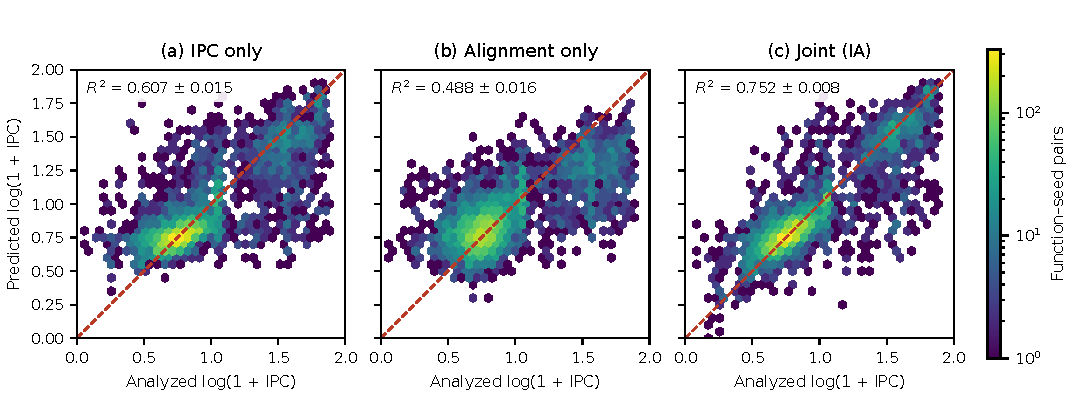
\includegraphics[width=0.92\textwidth]{figures/ablation_prediction.pdf}
\caption{Effect of supervision on source-level IPC prediction. Each panel shows the same 2,000 test functions under all three training seeds, giving 6,000 function--seed prediction pairs. The source architecture and 9,762-update budget are fixed. Hexagon counts use a common logarithmic color scale; the dashed line denotes exact prediction. Annotations report mean $\pm$ sample SD of individual-seed $\Rsq$. All predictions are included.}
\label{fig:supervision}
\end{figure*}

\paragraph{Assembly encoding.}
IA improves transformed-target $\Rsq$ from 0.734 with BPE to 0.752, an absolute gain of 0.018. It also reduces MAE from 0.293 to 0.280, or 4.4\%. IA has higher transformed-target $\Rsq$ at all three matched seeds. Since the source architecture and readout are unchanged, this comparison demonstrates that the assembly representation used during training affects the quality of source-only prediction.

The tokenization statistics illustrate how the representations allocate their sequence budget. Before truncation, training assembly has a mean length of 584.6 tokens under BPE and 107.4 under IA. With the common 512-position cap, 36.60\% of training assembly sequences exceed the limit under BPE, compared with 2.35\% under IA. IA therefore presents a more complete instruction stream within the same positional budget.

IA reduces the assembly vocabulary from 16,384 entries to 254, bringing the joint training model from approximately 15.04M to 10.91M parameters. Both models retain the same 7.52M-parameter source encoder for prediction. The assembly-side design therefore improves the learned predictor while preserving the source-side model size.

\subsection{Supervision Across Encoders}
We compare IPC-only and joint supervision within each source encoder. The compact Transformer and the two pretrained encoders span different model sizes and initialization strategies. Each comparison retains its source architecture and prediction readout, isolating the change in training supervision.

\paragraph{IPC-only adaptation.}
Under the same 9,762-update budget, IPC-only fine-tuning gives CodeBERT $\Rsq=\CBIPCRCell$ and UniXcoder $\Rsq=\UXIPCRCell$, with IPC MAE of \CBIPCMAE{} and \UXIPCMAE{}, respectively. The compact encoder is trained from scratch on the task corpus and uses approximately 6\% of either pretrained encoder's parameters.

\paragraph{Assembly supervision beyond the compact encoder.}
Adding assembly alignment raises CodeBERT's mean $\Rsq$ from \CBIPCR{} to $\CBJointRCell$ and reduces MAE from \CBIPCMAE{} to \CBJointMAE{}. All three matched seeds improve, with absolute $\Rsq$ gains of 0.008--0.023. Source architecture, learning rate, training examples, updates, and readout remain fixed, extending the supervision benefit to a broadly pretrained representation.

On the fixed 2,000-function sample, UniXcoder reaches $\Rsq=\UXJointRCell$ with joint supervision and \UXIPCR{} with IPC-only adaptation. Its joint MAE is \UXJointMAE{}, compared with \UXIPCMAE{}. The matched-seed $\Rsq$ changes are $+0.004$, $+0.006$, and $-0.006$. Section~\ref{sec:expanded} evaluates these frozen models on the complete test partition and its training-overlap-filtered subset.





\begin{newtext}
\paragraph{Feature and assembly references.}
Table~\ref{tab:reference} places the source model against simple feature baselines on the same 2,000 test functions. Hand-written source counts with gradient boosting reach $\Rsq=0.475$ with the 5,000-function readout sample and 0.585 with all 309,913 training functions. The learned source model reaches 0.752 after encoder training on all 309,913 functions and Ridge fitting on 5,000 embeddings. Source counts with Ridge reach 0.067. These comparisons show the benefit of learned source representations over the evaluated structural counts.

Assembly category counts with gradient boosting reach $\Rsq=0.906$, and an assembly-input IA Transformer reaches $0.919\pm0.003$. These references connect the source-query task to the compiled view used for supervision.

\end{newtext}

\begin{table}[t]
\begin{newtext}
\caption{\new{Feature and assembly-input references. All use the same 2,000 test functions; $\Rsq$ is on $\log(1+\mathrm{IPC})$ and MAE is in IPC units. ``5k'' and ``all'' denote labeled training samples. The Transformer uses all training functions for encoder training and 5k for Ridge; its scores summarize three seeds.}}
\label{tab:reference}
\centering\small
\setlength{\tabcolsep}{3pt}
\begin{tabular}{lcc}
\toprule
Prediction input / model & $\Rsq$ & MAE\\
\midrule
\multicolumn{3}{l}{\textit{Source input}}\\
Counts, Ridge (all) & .067 & .634\\
Counts, GBM (5k) & .475 & .431\\
Counts, GBM (all) & .585 & .376\\
\midrule
\multicolumn{3}{l}{\textit{Assembly input}}\\
Instruction count, GBM (all) & .140 & .565\\
Category counts, GBM (all) & .906 & .150\\
IA Transformer & .919 $\pm$ .003 & .1313 $\pm$ .0005\\
\bottomrule
\end{tabular}
\end{newtext}
\end{table}

\begin{newtext}
\subsection{Missing Declaration Context}
The mixed-view model reaches $\Rsq=0.660\pm0.012$ on declaration-stripped inputs, with IPC MAE 0.317 (Table~\ref{tab:incomplete}). On complete inputs for the same 1,136 functions it reaches $0.681\pm0.002$. Across all 2,000 complete test functions it retains $\Rsq=0.739\pm0.003$, compared with 0.752 for the original joint model. Prediction operates directly on source and remains available for stripped functions that fail compilation checks. Mixed-view training supports this use while largely preserving performance on complete inputs.

The transformation reduces mean source length from 323.6 to 190.8 BPE tokens and lowers the compilation-check pass rate from 100\% to 2.8\%. The original model, trained exclusively on complete inputs, obtains $\Rsq=-0.718\pm0.071$ on declaration-stripped inputs. Exposure to both input forms during training restores prediction quality under this input change. Adding declaration-stripped inputs to the Ridge fitting observations yields mean $\Rsq=0.665$, close to the 0.660 obtained with complete-view readout fitting. The primary result therefore uses the same complete-view Ridge protocol as the other neural models.

\end{newtext}

\begin{table}[t]
\begin{newtext}
\caption{\new{Complete and declaration-stripped inputs for the same 1,136 test functions; the first column covers all 2,000 test functions. $\Rsq_{\log(1+y)}$, mean $\pm$ sample SD over three seeds, Ridge fitted on complete inputs. Mixed-view training uses $p=0.5$. Only 2.8\% of declaration-stripped inputs pass compilation checks.}}
\label{tab:incomplete}
\centering\small
\setlength{\tabcolsep}{3pt}
\begin{tabular}{lccc}
\toprule
Training & Complete & Complete & Stripped\\
 & (2,000) & (1,136) & (1,136)\\
\midrule
Original joint model & .752 $\pm$ .008 & .704 $\pm$ .008 & $-$.718 $\pm$ .071\\
Mixed-view model & .739 $\pm$ .003 & .681 $\pm$ .002 & .660 $\pm$ .012\\
\bottomrule
\end{tabular}
\end{newtext}
\end{table}



\subsection{Full Partition and Training Overlap}
\label{sec:expanded}
Table~\ref{tab:expanded} extends the paired supervision comparison to all 17,301 test functions. Joint supervision raises $\Rsq$ from 0.889 to 0.900 for CodeBERT, from 0.909 to 0.914 for UniXcoder, and from 0.593 to 0.759 for the compact encoder. Each encoder also improves in mean IPC MAE and Spearman $\rho$. The larger evaluation therefore extends the supervision benefit to the pretrained encoders in both numerical error and target ordering.

Filtering removes 4,701 training-near-duplicates, leaving 12,600 functions. Of the full test partition, 1,212 functions have identical lexical token sequences to training inputs after comment and whitespace removal. On the retained subset, joint supervision raises $\Rsq$ from 0.828 to 0.843 for CodeBERT, from 0.858 to 0.866 for UniXcoder, and from 0.493 to 0.661 for the compact encoder. All three encoders improve at every matched seed on both the full partition and the filtered subset. The absolute gains on the filtered subset range from 0.012 to 0.021 for CodeBERT, 0.002 to 0.013 for UniXcoder, and 0.160 to 0.171 for the compact model.

IA also remains ahead of BPE when evaluation expands: compact joint $\Rsq$ increases from 0.748 to 0.759 on the full partition and from 0.645 to 0.661 after filtering. Spearman $\rho$ improves from 0.787 to 0.797 and from 0.708 to 0.722, respectively. Across filtering thresholds 0.8, 0.9, and 0.95, the ordering of supervision conditions and the advantage of IA over BPE remain unchanged. Joint supervision improves each matched seed for all three encoders at every threshold. These results connect the controlled ablations to a larger evaluation with reduced training overlap.

\begin{table*}[t]
\caption{Expanded evaluation with frozen encoders and the fixed 5,000-function Ridge fitting set. The filtered subset excludes training-near-duplicates at normalized token 5-gram Jaccard similarity $\geq0.9$. Values are mean $\pm$ sample SD over three seeds. $\Rsq$ uses $\log(1+\mathrm{IPC})$, MAE is in IPC units, and $\rho$ is Spearman correlation.}
\label{tab:expanded}
\centering\small
\setlength{\tabcolsep}{4pt}
\begin{tabular}{lcccccc}
\toprule
 & \multicolumn{3}{c}{Full test partition (17,301)} & \multicolumn{3}{c}{Filtered subset (12,600)}\\
\cmidrule(lr){2-4}\cmidrule(lr){5-7}
Encoder / supervision & $\Rsq$ & MAE & $\rho$ & $\Rsq$ & MAE & $\rho$\\
\midrule
CodeBERT / IPC & $.889\,\pm\,.003$ & $.157\,\pm\,.002$ & $.876\,\pm\,.004$ & $.828\,\pm\,.005$ & $.178\,\pm\,.002$ & $.816\,\pm\,.006$\\
CodeBERT / joint & $.900\,\pm\,.002$ & $.150\,\pm\,.002$ & $.884\,\pm\,.001$ & $.843\,\pm\,.003$ & $.170\,\pm\,.002$ & $.8253\,\pm\,.0003$\\
\midrule
UniXcoder / IPC & $.909\,\pm\,.003$ & $.143\,\pm\,.001$ & $.896\,\pm\,.002$ & $.858\,\pm\,.005$ & $.163\,\pm\,.001$ & $.843\,\pm\,.003$\\
UniXcoder / joint & $.914\,\pm\,.001$ & $.142\,\pm\,.001$ & $.898\,\pm\,.001$ & $.866\,\pm\,.001$ & $.160\,\pm\,.002$ & $.847\,\pm\,.002$\\
\midrule
Compact / IPC & $.593\,\pm\,.009$ & $.338\,\pm\,.005$ & $.687\,\pm\,.006$ & $.493\,\pm\,.008$ & $.326\,\pm\,.005$ & $.606\,\pm\,.004$\\
Compact / joint (BPE) & $.748\,\pm\,.003$ & $.253\,\pm\,.001$ & $.787\,\pm\,.002$ & $.645\,\pm\,.004$ & $.264\,\pm\,.001$ & $.708\,\pm\,.003$\\
Compact / joint (IA) & $.7588\,\pm\,.0004$ & $.244\,\pm\,.001$ & $.797\,\pm\,.002$ & $.661\,\pm\,.002$ & $.2575\,\pm\,.0004$ & $.722\,\pm\,.003$\\
\bottomrule
\end{tabular}
\end{table*}

\subsection{Inference Cost}
\label{sec:cost}
Table~\ref{tab:cost} measures the retained prediction paths on one A100. The compact encoder and scalar readout take 1.79\,ms per pretokenized query, compared with 8.98\,ms for CodeBERT and 8.92\,ms for UniXcoder. At batch size 16, the compact path processes 2,250 functions per second, compared with approximately 168 for either pretrained encoder. Peak allocated memory at batch size 1 is 48.7\,MiB, compared with 500.4\,MiB and 505.2\,MiB. The compact instantiation thus provides approximately fivefold lower single-query latency and thirteenfold higher batched throughput under this measurement configuration.

Separately measured host tokenization averages 0.34\,ms per function for the compact tokenizer, 0.83\,ms for CodeBERT, and 0.95\,ms for UniXcoder.

\begin{table}[t]
\caption{Source encoder plus scalar linear readout on the same A100, in float32 with 512-token padded inputs. Latency is the mean at batch size 1; throughput uses batch size 16. Memory is peak PyTorch-allocated GPU memory at batch size 1. Tokenization and transfers are excluded.}
\label{tab:cost}
\centering\small
\setlength{\tabcolsep}{3pt}
\begin{tabular}{lccc}
\toprule
Encoder & Latency (ms) & Throughput (fn/s) & Memory (MiB)\\
\midrule
CodeBERT & 8.98 & 168 & 500.4\\
UniXcoder & 8.92 & 168 & 505.2\\
Compact & 1.79 & 2250 & 48.7\\
\bottomrule
\end{tabular}
\end{table}

\section{Discussion}
\subsection{A Source Interface to Static Analysis}
The framework makes compilation-derived information available through a source query, supporting function inspection when surrounding build context is unavailable. Mixed-view training extends this interface to excerpts with missing declarations. Complete and stripped inputs retain the original implementation label, linking the available source to its analyzed static IPC.

\subsection{What the Compiled View Contributes}
Paired assembly associates source constructs with implementation structure beyond a scalar IPC label. IA exposes recurring instruction patterns and more of each implementation within the sequence budget. The supervision and tokenization comparisons show how this additional training view improves the source representation.

\subsection{Supervision Across Representations}
The paired-view principle benefits both task-trained and pretrained source encoders, with gains persisting after training-overlap filtering. Their different effect sizes show that assembly supervision can accompany different starting representations. The framework also supports different deployment costs: the compact instantiation provides lower encoding latency and memory use, while pretrained variants provide higher predictive accuracy.

\section{Threats to Validity}
\label{sec:threats}
The target is static IPC under one compilation and processor-analysis configuration. \llvmmca{} analyzes 100 iterations without following input-dependent control flow or executing callees. Hardware-measured throughput can differ from analyzer estimates~\cite{chen2019bhive,renda2020difftune}; additional compiler and processor settings would test configuration transfer.

Training-overlap filtering evaluates sensitivity to lexical similarity; the retained subset also changes in composition. Project-disjoint evaluation would test transfer across code origins~\cite{bock2023domain}. Three seeds measure training variation within these fixed data partitions. The ablations quantify objective contributions under the selected joint configuration, while feature references cover the specified counts and model families.

Mixed-view results concern one declaration-removal rule and mixing probability. An augmented IPC-only control would isolate assembly supervision's contribution to that adaptation. Pretrained models incorporate prior code pretraining beyond the shared task-training budget. Efficiency measurements concern float32 source encoding and linear prediction on one GPU, excluding tokenization and transfers.

\section{Conclusion}
Joint source--assembly alignment and IPC regression transfer implementation information into source-level static performance predictors. Controlled ablations show the value of both training objectives, while IA improves assembly coverage and the resulting source representation. Prediction retains only the source encoder and a linear readout.

On all 17,301 test functions and the 12,600-function training-overlap-filtered subset, joint supervision improves $\Rsq$ at every matched seed for the compact encoder, CodeBERT, and UniXcoder. The compact instantiation also provides a low-cost prediction path, taking 1.79\,ms per pretokenized query on an A100. Mixed-view training extends source prediction to excerpts with missing declarations, reaching $\Rsq=0.660$ on 1,136 declaration-stripped functions. Paired compiled implementations therefore supply reusable training information for source-level static performance estimation, including inputs whose available context does not support independent compilation.

\bibliographystyle{IEEEtran}
\bibliography{references}

\end{document}
